%  This is the main thesis tex file.  It will assemble the separate source
%  files into a document.  It is intended to be built by the supplied Makefile.
%  Author:  Anthony Gervasi
%
%  Usage:  type 'make' in the command shell
%  Requirements:  Tex installed, Linux/Unix environment


\documentclass[13pt]{ucthesis}

\usepackage{url}
\usepackage{pstricks,pst-node,pst-text,pst-3d}
\usepackage{amsmath}
\usepackage{mathrsfs}
\usepackage{amssymb}
\usepackage{graphics}
\usepackage{epsfig}
\usepackage{fancyhdr}
\usepackage{auto-pst-pdf}
\usepackage{cite}
\usepackage{nomencl}
 \usepackage{subfigure}% subcaptions for subfigures
 \usepackage{subfigmat}% matrices of similar subfigures, aka small mulitples

\author{Brian Fehrman}
\title{Experiments on Time Reversal Focusing of Acoustic Energy at a Crack Location in One Dimension}
\degreeyear{2012}

\setlength\topmargin{-0.5in}
\setlength\oddsidemargin{0.45in}

\makeglossary

\begin{document}


\maketitle

\begin{frontmatter}
\begin{abstract}
% Abstract follows
A large number of micro-meteoroids speed towards the earth each day. In addition, a substantial amount of debris orbits the earth. Lightweight space structures and satellites are often at the mercy of these speeding objects. Collision is not always avoidable and surface damage is almost inevitable which is very costly to repair once it occurs. Self healing materials that can automatically repair themselves once damaged are of interest to this area. The healing process is in competition with the crack expansion process and it may be necessary to accelerate the healing process in order to achieve sufficient mechanical recovery. Focused acoustic energy is one theorized way to increase the recovery rate. Time reversal signal processing is an algorithm which can focus acoustic energy at an arbitrary crack location. In this work time reversal acoustic focusing in one dimension at a defect with an unknown location was explored. It was shown that the time reversal process is able to achieve a localized focusing of acoustic stress waves at a crack location in both nylon and steel rods. The experimental results were compared with theoretical calculations and a decent match was seen. Crack detection tests were also performed and it was shown that the program could detect when damaged occurred within the system.

  % You may enter in the file or directly here.
\end{abstract}
\printglossary
\tableofcontents
\listoffigures
%\listoftables
\end{frontmatter}



% You will need to add chapter and input lines for your own work.
%  The following give some examples:

\chapter{Introduction}\label{ch:Introduction}

% Introduction

Each day, more than 100 billion meteoroids larger than a microgram come speeding through Earth's atmosphere \cite{Close2010}. A large number of debris objects are presently in orbit around the earth (see Figure \ref{fig:orbitalDebris}). NASA states that there are over 21,000 debris objects larger than a softball, 500,000 particles larger than a marble, and over 100 million smaller pieces that cannot be tracked. Due to the large number of objects traversing the space surrounding earth, it is likely that impact will occur with lightweight, low orbiting space structures and satellites which can result in varying degrees of damage \cite{NASAOD2012}. The most likely impact will come from the smallest pieces as they occur in the largest numbers and are hard to avoid since they are hard to detect. These smaller particles will cause damage in the form of surface cracks and abrasions. Technologies exist such as the Whipple Shield (or meteor bumper) which help to mitigate the effects of impacts by absorbing some of the energy or breaking larger objects into smaller pieces \cite{NASAHVIT2012}. However, it is still likely that particles can make it all the way to the underlying structure and cause damage which will build up over time. Access to these structures is difficult, costly, and dangerous. Repair missions will inevitably leave behind more debris which will increase the likelihood of future damage occurring to the structure being repaired as well as other structures in orbit. Materials with the ability to automatically heal damage as it occurs are very desirable for these applications \cite{Lee2009}.

\begin{figure}[ht!]
\centering
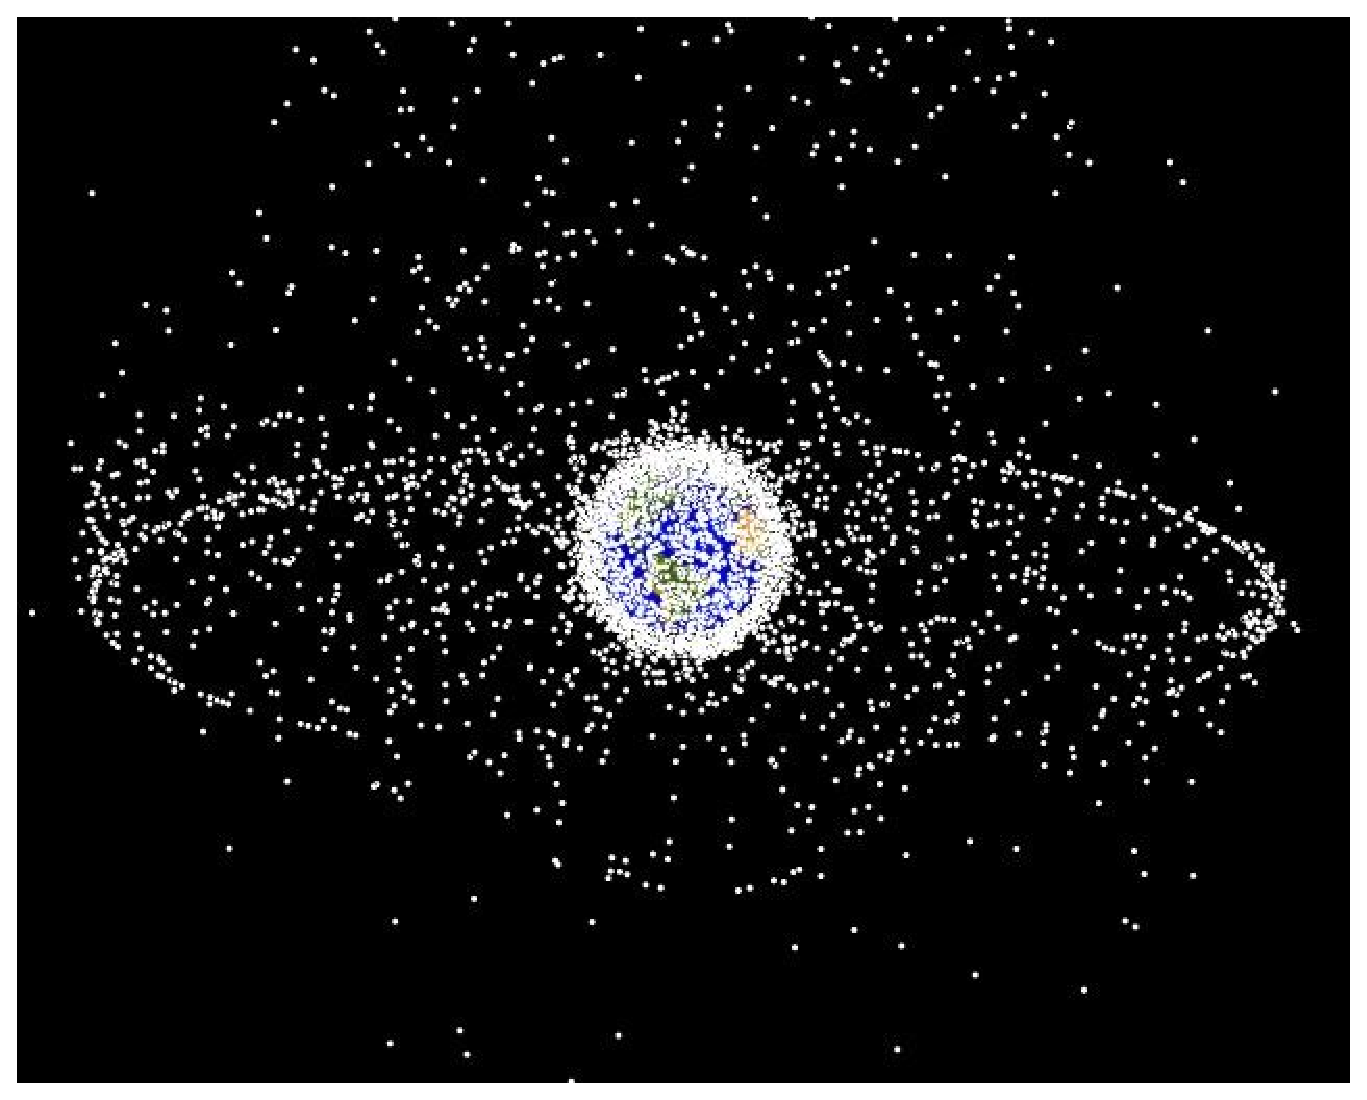
\includegraphics[width=0.8\textwidth]{eps_pics/orbitalDebris}
\caption{ Image from NASA which depicts the debris objects that are currently orbiting the Earth. Some examples of debris objects include: broken spacecraft, upper stages of launch vehicles, debris that is intentionally released from missions, debris from collisions, and paint flecks. Much of the debris seems benign due to its size but is made dangerous by its high velocity (up to 60km/s for smaller pieces).
\newline
imagesource:[http://orbitaldebris.jsc.nasa.gov/photogallery/beehives/GEO640.jpg]
	 \label{fig:orbitalDebris}} 
\end{figure}

\section{Self-Healing}

Crack healing in materials owes some of its early studies to Wool and O'Connor who modeled crack healing in polymers and experimented with cantilever beams \cite{Wool1981, Wool1982}. They found that polymer crack healing occurs in the following five stages: a) surface rearrangement, b) surface approach, c) wetting, d) diffusion, and e) randomization. Sloof, Song, and others have developed materials in which thermal activation caused a mending of cracks \cite{Song2009, Sloof2009, Bosman2009, Djugum2009, Luo2009}. Caruso et. al. reported on material strength recovery in thermoplastics by using solvent-based healing agents \cite{Caruso2009}. Inspired by the idea of biological entities being able to automatically heal wounds, a self-healing material was made by White et. al. in which a catalyst and microcapsules filled with a reactive fluid were distributed throughout a material \cite{White2001}. When the material was cracked, the capsules released their fluid which polymerized upon contacting the catalyst and effectively fused the faces of the crack together (Figure \ref{fig:selfHealingMedium}). Sottos et. al. have improved this self-healing implementation and found that damaged materials recovered up to 90\% of their original strength \cite{Sottos2009}. The White and Sottos group have also studied crack healing by introducing hardener filled microcapsules into an epoxy that was molded into a double cantilever beam fracture specimen \cite{Mcllroy2009}. This concept has been extended to a self-healing coating that contained epoxy filled microcapsules and was tested on cold rolled steel sheets with good results\cite{Zhao2012}. Manuel et. al. created a matrix containing wires that could apply a force to the material to close a crack and then the material was heated to weld the crack together \cite{Manuel2009}. Adhesives with self-healing properties have been created by Jin et. al. and tested on composite laminates where they were found to increase the life of specimens subject to fatigue \cite{Jin2009}. Self repairing chemicals have been successfully implemented on composite airplane components and were able to return to 88\% of their original strength after impact and shear testing \cite{Dry2009}. Recently, there has been a large interest in applying self-healing methods to help prolong the life of concrete which is very prone to cracks \cite{Wu2012}. 

\begin{figure}[ht!]
\centering
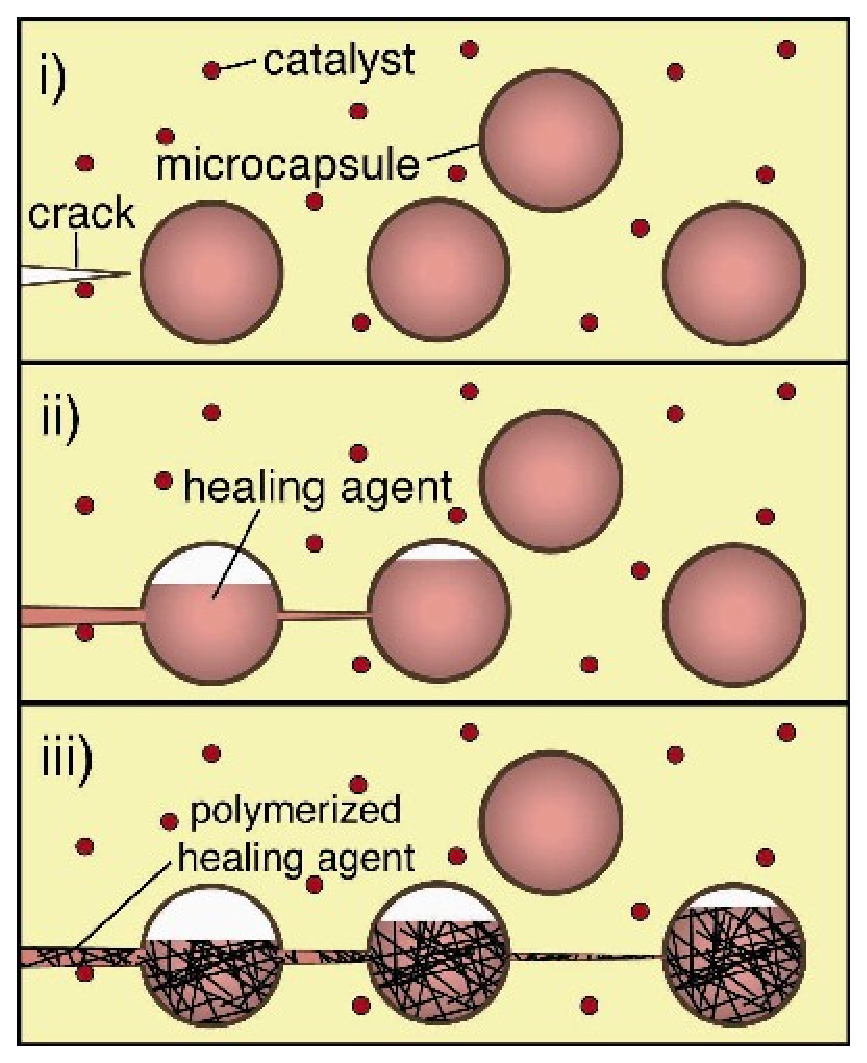
\includegraphics[width=0.5\textwidth]{eps_pics/selfHealingMedium}
\caption{ Concept drawing of a self-healing material in which microcapsules filled with a reactive fluid and a catalyst are spread throughout that material. The drawing depicts the stages of damage, fluid release, and polymerization.
\newline
source:[http://www.howstuffworks.com/self-healing-spacecraft1.htm]
	 \label{fig:selfHealingMedium}} 
\end{figure}

\section{Accelerating the Self-Healing Process}

Typically, the damaging process will continue to occur as the material attempts to mend itself together. It is therefore important that the material heals itself quickly so that the damage process does not dominate and prevent the material from reaching a full mechanical recovery. Studies have been performed on fatigue crack propagation in a self healing material \cite{Brown2003}. Sheng, Burattini, and many others reported on increasing the healing rate by improving the materials that are used \cite{Sheng2009, Burattini2009, Nakao2009, Imperiale2009, Zhang2007}. The use of U.V. light has been researched as a way to accelerate the healing process in metallopolymers and ethyl cellulose based copolymers \cite{Tang2009, Burnworth2009}. Wool and O'Connor found in their work that an increase in pressure at the crack interface during the early stages of healing or an increase in temperature at any stage can increase the rate at which the material recovers \cite{Wool1981}. Murphy et. al. have studied direct heating as a method to increase healing capabilities\cite{Murphy2009}. Direct heating to improve healing has also been applied to concrete \cite{Garcia2009, Nishiwaki2009}. Applying pressure to a crack location via acoustic energy was studied by Korde et al. both theoretically and experimentally which found that acoustic energy can accelerate the healing process \cite{Sarrazin2009, Cushman2012, Barnes2009}. Fettig et. al. have also found that healing is optimized by ensuring good mixing in the early stages which can be brought about by localized pressure \cite{Fettig2009}. Sarrazin treated cracked nylon dog-bone specimens with ultrasonic probes which increased the temperature within the specimen and caused a fusing of the crack faces  \cite{Sarrazin2-2009}. By using ultrasonic waves both the temperature and pressure at a recovery site could be increased which results in a faster healing time.

\section{Implementation}

Two main problems arise when implementing any of the previously described external stimulation methods to accelerate the healing process; i) detecting when damage has actually occurred and ii) applying the stimulation energy only to the damage location. In regards to i), it would be highly inefficient and potentially damaging to continually introduce energy if healing is not taking place. Along similar lines of reasoning, one would want only to apply energy to the actual recovery location for increased efficiency and so that unintended damage to the system does not occur. Acoustic energy is the method chosen here as it offers solutions to both problems. 

\subsection{Damage Sensing}

Picture a rod with transducers on either end that are capable of playing and recording sound. First, one transducer propagates a low energy acoustic stress-waves through the material and the other records the response of the material. If this process is repeated periodically and the response is monitored then a change in the response is observed if there is a change in the medium (e.g., damage has occurred; Figure \ref{fig:detectChange}). The acoustic energy could then be applied after this change in response has been detected and cease once the system determines that the response has returned to its initial state within some tolerance level. Imaging using ultrasonics has been around for some time now and is probably most recognized in ultrasounds that are used during pregnancy \cite{Ultrasound2006}. Ultrasonic imaging has been widely used in nondestructive testing to find cracks within structures. Harris et. al. used acoustic emission to monitor the fatigue crack growth in both aluminum and steel samples \cite{Harris1974}. Detecting cracks in concrete by using ultrasound was reported by Zinin et. al. \cite{Zinin2000}. Acoustic waves have also been used to detect cracks in very fragile materials such as eggshells \cite{DeKetelaere2000}. Recently, ultrasound has been used in dentistry to detect microcracks within teeth \cite{Matsushita2012}.

 \begin{figure}[ht!]
\begin{subfigmatrix}{2}
\subfigure[Acoustic wave propagating through medium with no defect]
{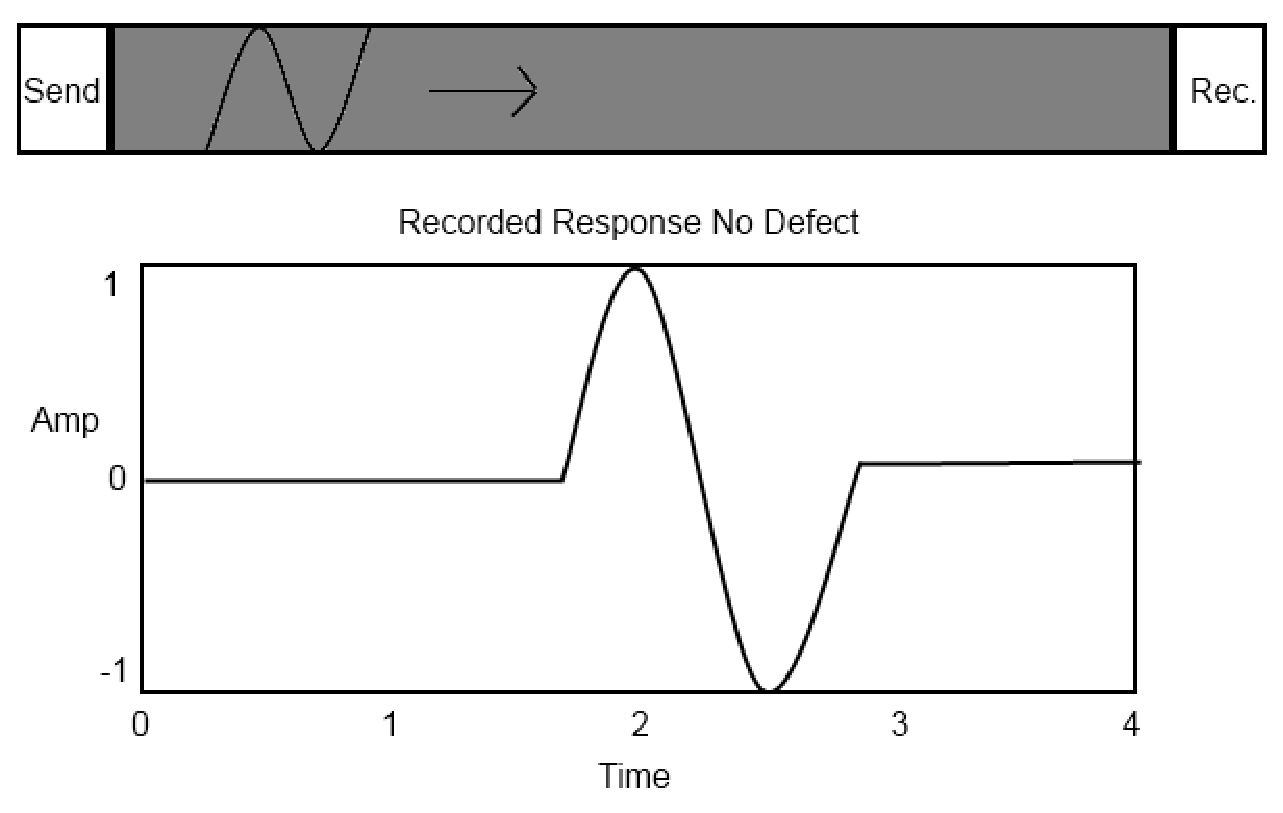
\includegraphics[width=0.5\textwidth]{eps_pics/sentNoCrack}}
\subfigure[Acoustic wave propagating through medium with a crack]
{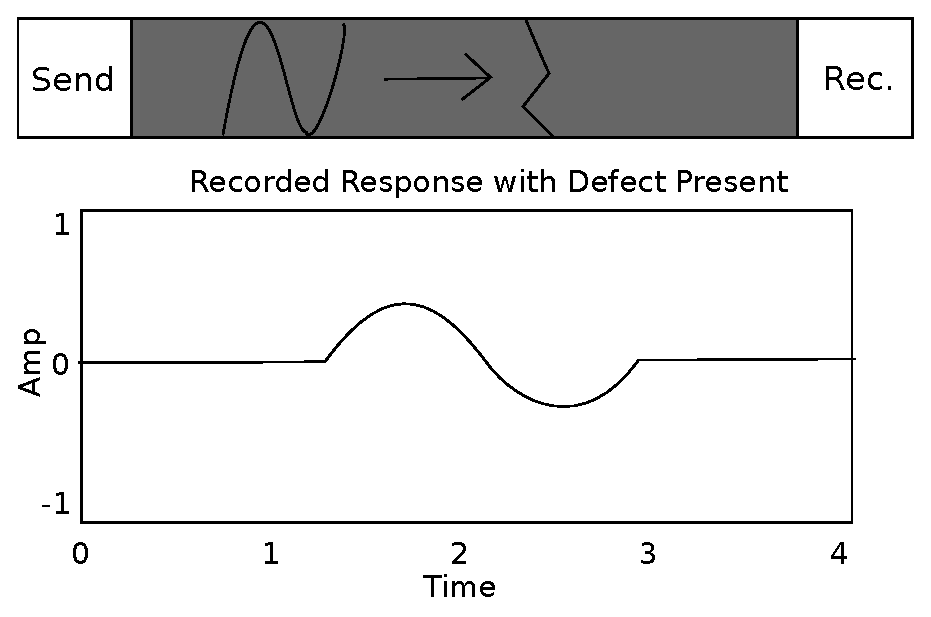
\includegraphics[width=0.5\textwidth]{eps_pics/sentCrack}}
\end{subfigmatrix}

   \caption
   { \label{fig:detectChange}
   a)A transducer sends an acoustic wave through a medium and a transducer on the opposite end records the response. This material is seen without a defect and the simulated response is shown; b) Same as a), but a defect is now present in the medium which causes a change in the response recorded on the opposite end and is seen in the simulated recorded response.
 }
\end{figure}

\subsection{Time Reversal Focusing}
Besides the mechanics of focusing the energy at the crack location, the problem arises that the location of the defect is not necessarily known. A method is needed that not only localizes the energy at the healing site but it does so without knowledge of the physical location of that site. Acoustic time reversal signal processing is one such method that possesses the aforementioned qualities. Picture again the cracked medium with transducers on either end. As before, a stress-wave is played by one transducer. This time, however, both transducers record signals. The stress-wave propagates through the medium and strikes the crack which causes the wave to split into multiple components that transmit to the opposite transducer and reflect back to the original sending transducer where they are recorded. If the transducers re-amplify and playback these signals in a time reversed fashion then the waves meet at the point where they split (here, the crack) which causes a focusing of their energy at that point. The focused wave splits again into multiple components that are recorded by each transducer and the time reversal process is repeated iteratively with a better focusing being achieved on each iteration until limits due to dissipation are reached (Figure \ref{fig:trDrawing} illustrates this concept). The time reversal concept can be extended to multiple dimensions in which the transducers are placed around the boundary. In a self-healing material, the focusing of energy at a crack location would accelerate the healing process at that site.

\begin{figure}[ht!]
\centering
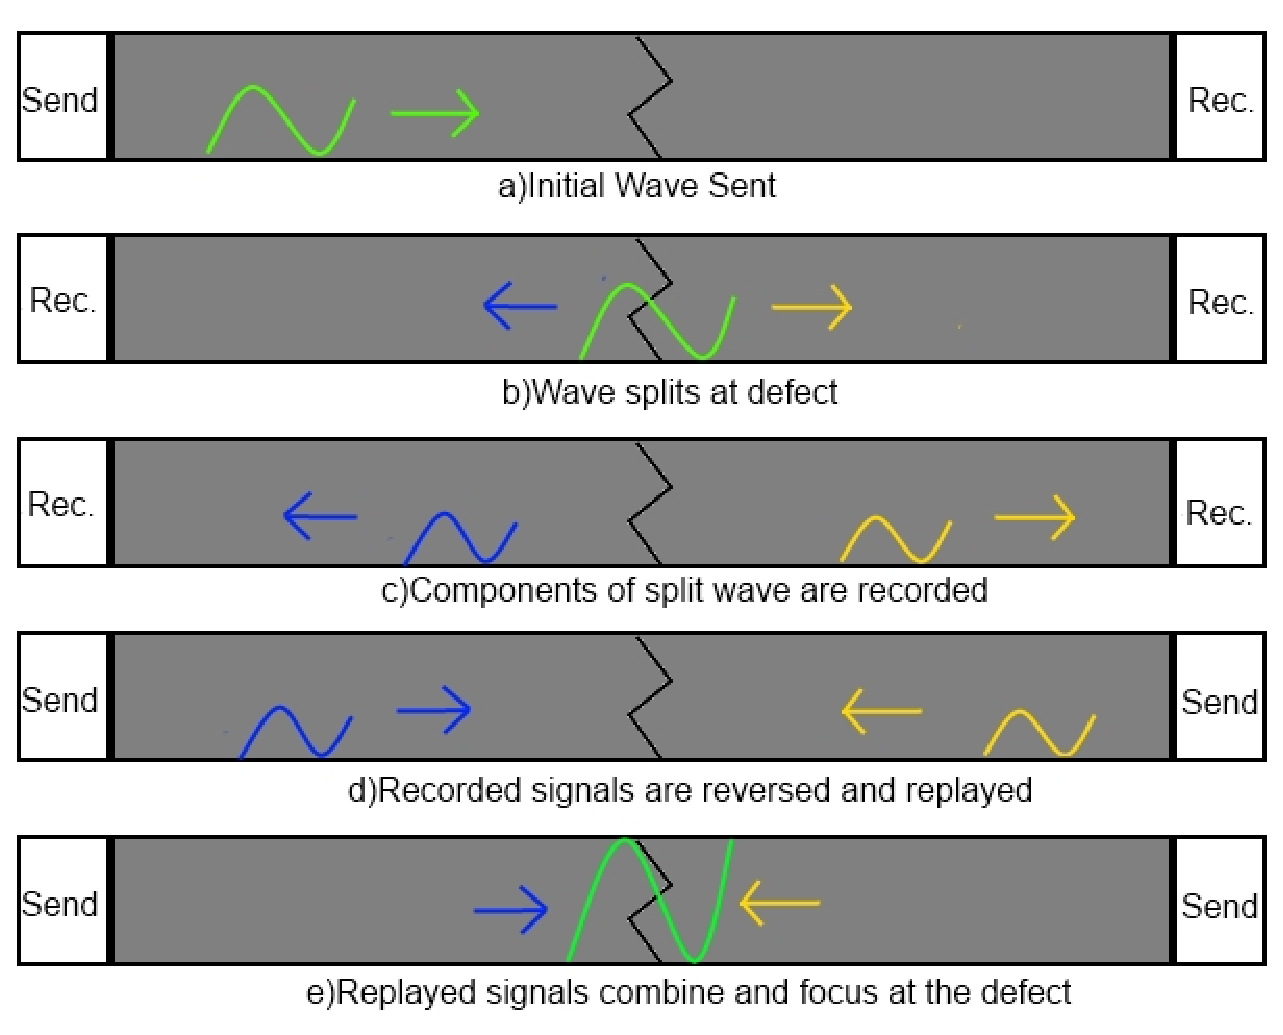
\includegraphics[width=0.7\textwidth]{eps_pics/trDrawing}
\caption{ Concept drawing of time reversal in one dimension; a) An initial wave is sent out by a transducer; b) The wave travels down the rod until it hits the crack and splits into multiple components; c) The components of the incident wave travel towards each transducer where they are recorded; d) The recorded signals are amplified and replayed in a time reversed fashion; e) The wave components simultaneously reach the crack location where they first split and combine to cause a focusing of their amplitude at that point.
	 \label{fig:trDrawing}} 
\end{figure}

Mathematically, time reversal is the time domain analog of phase conjugation which has been used in adaptive optics to correct for wavefront phase aberrations by forming a mirror to produce the conjugate phase aberrations of the incoming wave which results in a corrected wavefront \cite{Pepper1982}. Acoustic time reversal has been studied extensively by Fink et. al. in which he first setup an array of transducers to send and receive ultrasonic waves through a rubber medium with random thicknesses and a hydrophone embedded as a reflector/receiver.  Fink also has shown iterative focusing by experimenting with an array of transducers and two metal wires as reflectors. In the iterative experiments, it was shown that the energy focused on the strongest reflector after successive iterations \cite{Fink1993}. Experiments were performed by Derode et. al. in which a transducer played a signal through a liquid containing over 2000 rods and an array of transducers located on the opposite side of the rods played the captured signals back and it was found that the replayed signals converged on the original source \cite{Derode1995}. Time reversal has been applied to acoustic communications in both the ocean and air to achieve better signal to noise ratio by focusing the signal at the desired receiver \cite{Smith2003, Song2012, Shimura2012}. Great promise has also been shown with applying time reversal to biomedical application such as the focusing of ultrasonic waves to destroy kidney stones or hyperthermia brain treatment \cite{Fink2003}. The concept of time reversal is not only applicable to acoustics but can also be used with electromagnetic waves \cite{Lerosey2004}. Liu et. al. have shown experimentally that bit-rate-errors in radio communications can be reduced by applying time reversal \cite{Liu2008}. MIT has effectively created a microwave cannon by using the time reversal process to focus microwave energy \cite{Davy2010}.

\section{Objectives}
The overall goal, as devised by Dr. Korde, is to use time reversal acoustic focusing to accelerate the crack recovery process of a self-healing polymer by locally increasing the temperature and pressure. The work presented here looks at a subsection of that project which is the time reversal focusing at a crack location. There has been much theoretical and experimental work performed on applying time reversal in multiple dimensions. Here, the case of time reversal in one dimension is explored. Fouque et. al. performed calculations and simulations on one dimensional time reversal in random media with an embedded reflector to determine the reflector's location \cite{Fouque2006}. Korde performed calculations on focusing at a crack with piezoelectric transducers and time reversal processing \cite{Fehrman2012}. To the author's knowledge, time reversal focusing at a defect location in one dimension has not been performed experimentally. In this work experiments are performed on circular steel and nylon rods with piezoelectric transducers to send and receive signals. This could have direct applications to the rods used in deployable space structures that may become cracked over time. Although the analysis is eased in this scenario, there are difficulties introduced in performing the experiments in one dimensional structures of finite length that are not present when performing time reversal in multiple dimensions. For instance, it is required that a transducer both sends a signal and reads a signal in the same iteration such that the ringing of the transducer may interfere with the signal being read.\newline

The specific objectives of this work are to show:
\begin{enumerate}
\item Modeling and experimental verification of acoustic time reversal crack focusing in one dimension
\item Experimental verification of acoustic crack detection in one dimension
\item Experimental verification of iterative focusing and convergence of acoustic time reversal crack focusing in one dimension
	\begin{enumerate} 
	\item Show that with each iteration, the amplitude seen at the defect increases until a convergence point is reached
	\end{enumerate}

\end{enumerate} % You may enter in the file or directly here.

\chapter{Modeling}\label{ch:Modeling}
% Modeling
This chapter begins with the models and derivations for the case of one dimensional time reversal and is based upon work performed by Korde \cite{Fehrman2012}. Following that material will be a brief overview of two dimensional time reversal which is drawn from a number of published sources.

\section{One Dimensional Wave Equation}
\label{sec:oneDWaveEquation}

In this section the one dimensional wave equation for a linear elastic material with uniform density and cross-sectional area will be derived. The derivation is based on knowledge from numerous books such as Kolsky \cite{Kolsky1963} and Brown et. al. \cite{Brown2008}.

\begin{figure}[ht!]
\centering
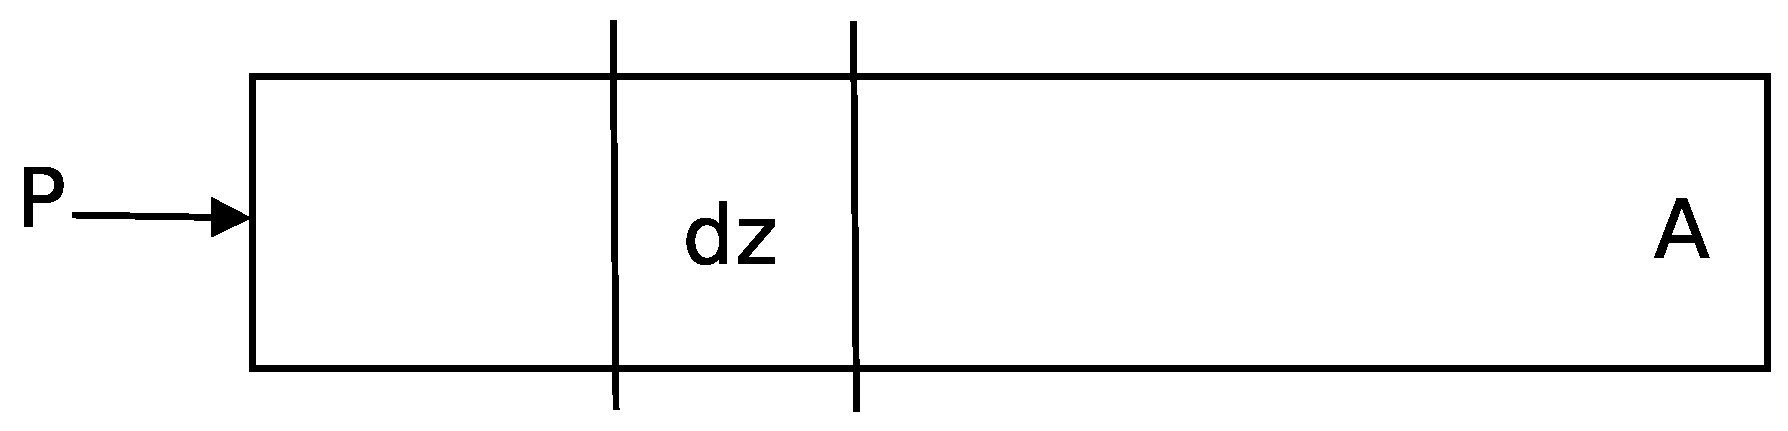
\includegraphics[width=0.8\textwidth]{eps_pics/deriveWaveRod}
\caption{Diagram for deriving the one dimensional wave equation given an axial pressure applied to one end of the material with uniform density and cross-sectional area.
	 \label{fig:deriveWaveRod}} 
\end{figure}

Figure \ref{fig:deriveWaveRod} gives a basic diagram that is used for the wave equation derivation, with $P$ being the axial pressure, $dz$ being the material's differential element of length, and $A$ being the cross-sectional area of the material. Define the stress in the z direction as:

\begin{equation}
T_3 = \frac{P}{A}
\end{equation}

\nomenclature{$P$}{Axial pressure applied to rod end}
\nomenclature{$A$}{Cross-sectional area of the rod}
\nomenclature{$dz$}{Differential element of length for the rod}
\nomenclature{$T_3$}{Stress in the z direction}

\begin{figure}[ht!]
\centering
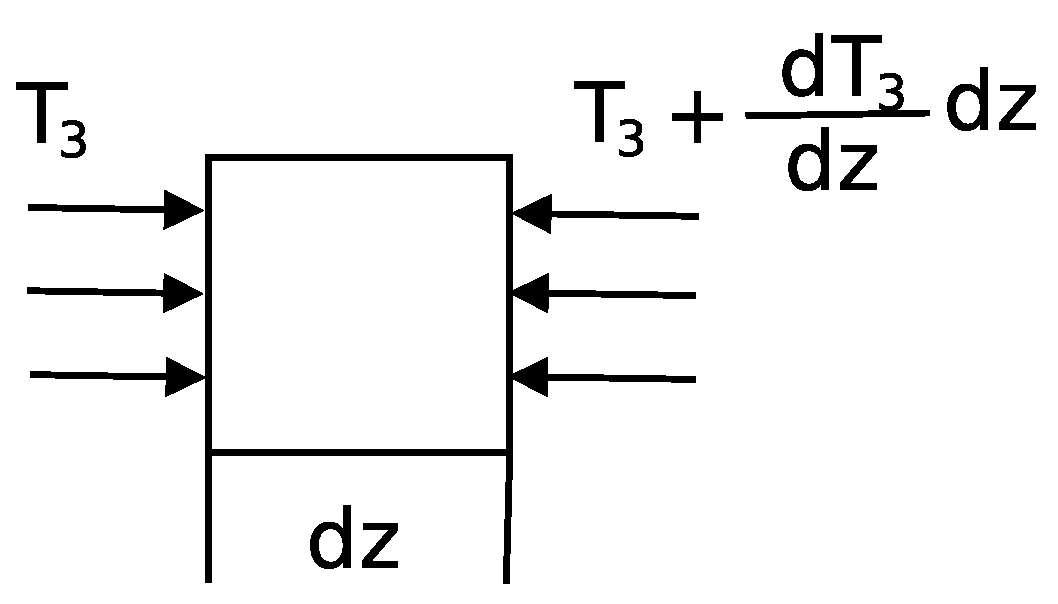
\includegraphics[width=0.8\textwidth]{eps_pics/diffElementRod}
\caption{Differential element showing the stresses acting on the rod.
	 \label{fig:diffElementRod}} 
\end{figure}

Applying Newton's second law and summing the forces,

\begin{equation}
-T_3A + (T_3 + \frac{dT_3}{dz}dz)A = A\rho^* dz \frac{d^2w}{dt^2}
\end{equation}

\nomenclature{$\rho^*$}{Density of the rod material}
\nomenclature{$w$}{Displacement of the rod}

With $\rho^*$ being the density of the rod material and $w$ being the displacement. Dividing through by the area,

\begin{equation}
-T_3 + T_3 + \frac{dT_3}{dz}dz = \rho^* dz \frac{d^2w}{dt^2}
\end{equation}

\begin{equation}
\frac{dT_3}{dz}dz = \rho^* dz \frac{d^2w}{dt^2}
\end{equation}

Canceling the $dz$ term,

\begin{equation}
\frac{dT_3}{dz} = \rho^* \frac{d^2w}{dt^2}
\label{eq:strainWave}
\end{equation}

$C^*_{33}$ is the elastic constant in the z direction and is defined as the ratio of the stress and strain in the z direction. This is given by,

\begin{equation}
C^*_{33} = \frac{T_3}{S_{33}} \implies T_3 = C^*_{33}S_{33}
\label{eq:T_3}
\end{equation}

\nomenclature{$C^*_{33}$}{Elastic constant in the z direction}
\nomenclature{$S_{33}$}{Strain in the z direction}

With $S_{33}$ being the strain in the z direction. Strain is the ratio of the change in material length to the original length and in this case is given by,

\begin{equation}
S_{33} = \frac{dw}{dz}
\label{eq:S_33}
\end{equation}

Inserting \ref{eq:S_33} in to \ref{eq:T_3} we see that

\begin{equation}
T_3 = C^*_{33}\frac{dw}{dz}
\label{eq:T_3fin}
\end{equation}

Putting \ref{eq:T_3fin} back in to \ref{eq:strainWave} and realizing that $w$ is a function of both $t$ and $z$,

\begin{equation}
C^*_{33}\frac{\partial ^2w}{\partial z^2} = \rho^* \frac{\partial ^2w}{\partial t^2}
\end{equation}

Dividing through by $\rho^*$ and moving the LHS term to the RHS, we arrive at

\begin{equation}
\frac{\partial ^2w}{\partial t^2} - c^{*2} \frac{\partial ^2w}{\partial z^2} = 0
\label{eq:waveEquationFin}
\end{equation}

\nomenclature{$c^*$}{Velocity of wave propagation through the rod}

With $c^*$ being the velocity of the wave propagation and is defined as,

\begin{equation}
c^* = \sqrt{\frac{C^*_{33}}{\rho^*}}
\end{equation}

\section{Piezoelectric transducers}

This section describes the governing equations for $d_{33}$ piezoelectric transducers that are placed on each end of a rod. The following work is based on derivations by Dr. Korde.

The constitutive equations for the transducers are:

\begin{equation}
T_3 = \overline{C_{33}} S_3 + \overline{d_{33}} D_3
\end{equation}

and 

\begin{equation}
D_3 = \overline{\epsilon ^T_{33}} E_3 + \frac{d_{33}}{s^E_{33}} S_3
\end{equation}

Where $D_3$, $E_3$, and $d_{33}$ are the electric displacement, electric field intensity, and the strain constant relating strain and field intensity, respectively, all in the z direction. The other variables are given by the following equations:

\begin{equation}
s^E_{33} = \frac{1}{C_{33}}
\end{equation}

\begin{equation}
\overline{C_{33}} = \frac{1}{s^E_{33}(1 - \frac{d^2_{33}}{s^E_{33}\epsilon ^T_{33}})}
\end{equation}

\begin{equation}
\overline{d_{33}} = -\frac{d_{33} / \epsilon ^T_{33}}{s^E_{33}(1 - \frac{d^2_{33}}{s^E_{33}\epsilon ^T_{33}})}
\end{equation}

\begin{equation}
\overline{\epsilon ^T_{33}} = -\frac{\epsilon ^T_{33}}{s^E_{33}(1 - \frac{d^2_{33}}{s^E_{33}\epsilon ^T_{33}})}
\end{equation}

With $C_{33}$ and $\epsilon ^T_{33}$ being the PZT elastic constant in the z direction and permittivity constant in the z direction respectively.

\begin{figure}[ht!]
\centering
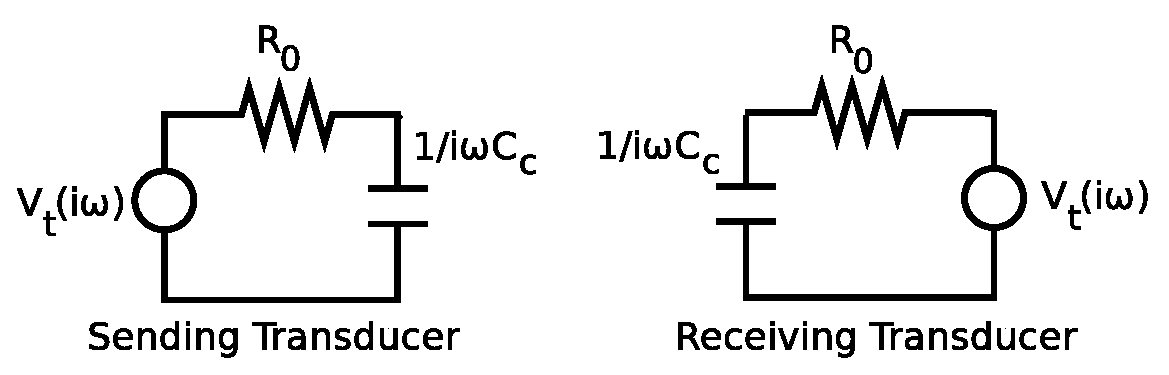
\includegraphics[width=1\textwidth]{eps_pics/trans_circ}
\caption{Equivalent circuit diagram for the piezoelectric transudcers.
	 \label{fig:trans_circ}} 
\end{figure}

The equivalent circuits for the transducers are modeled as a resistor and capacitor in series as shown in Figure \ref{fig:trans_circ} and with $C_c$ being the equivalent capacitance and is given by

\begin{equation}
C_c = \overline{\epsilon_{33}} \pi a^2/l
\end{equation}

Where $a$ and $l$ are the transducer area and length respectively. 

\section{Rod with Transducers}

\begin{figure}[ht!]
\centering
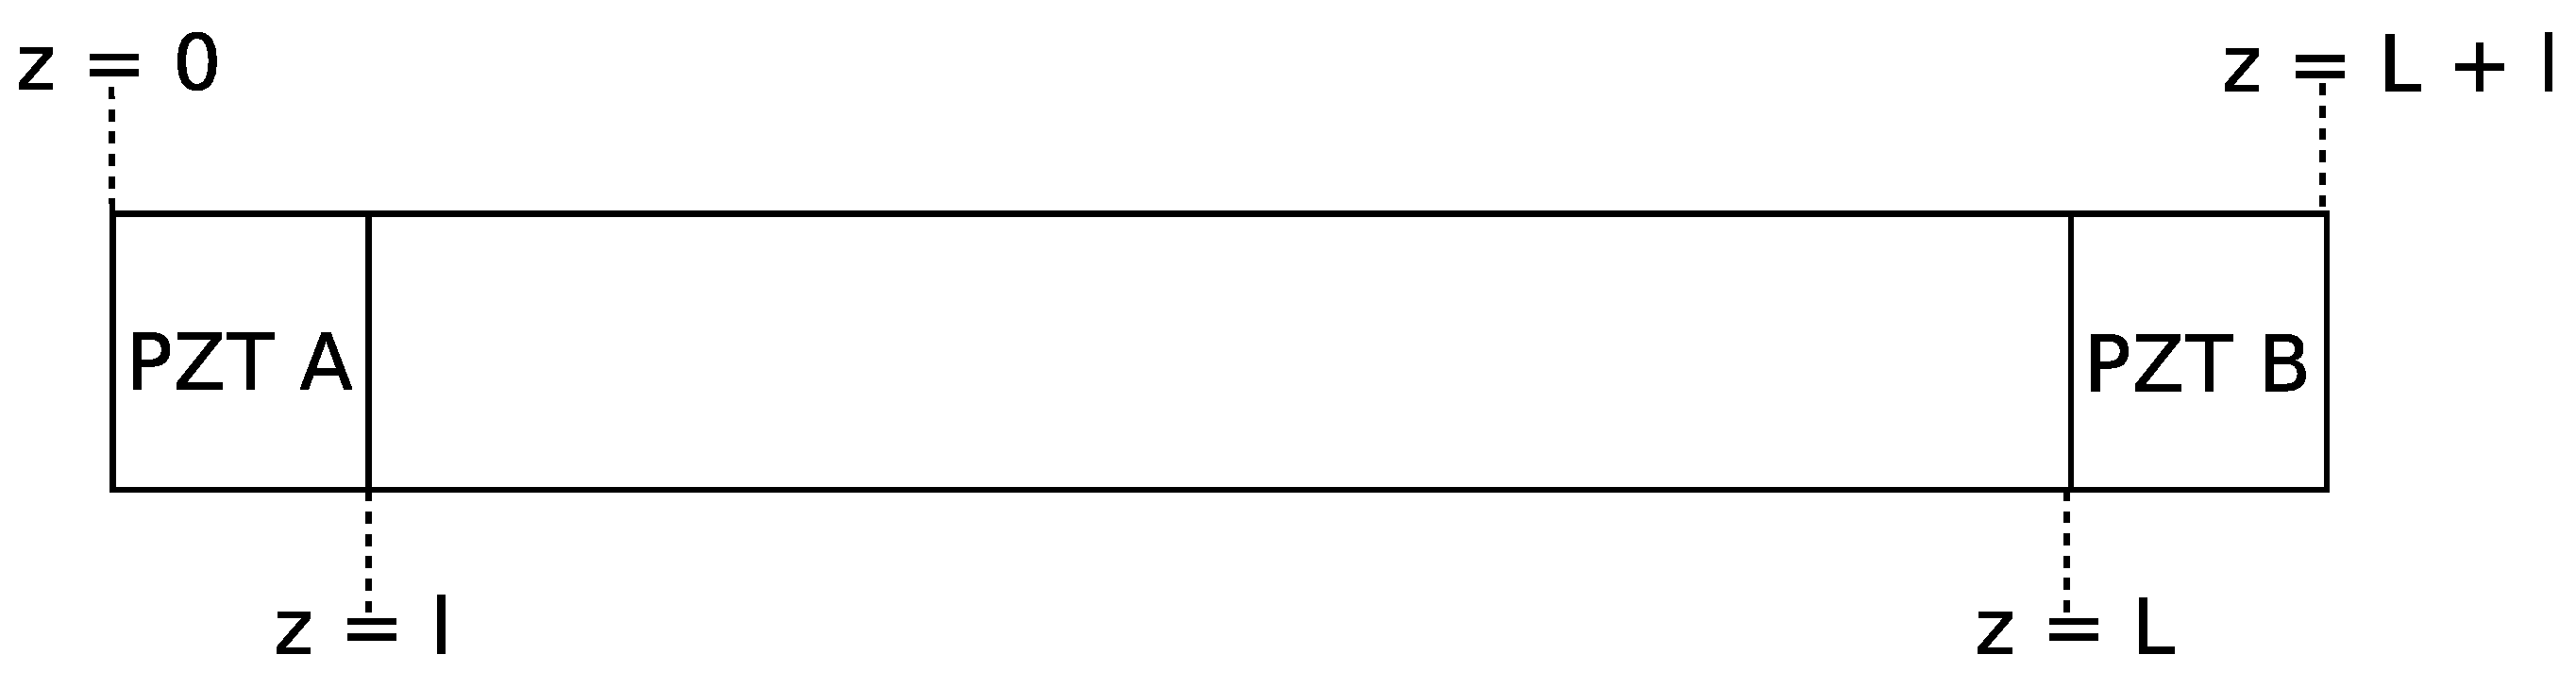
\includegraphics[width=0.8\textwidth]{eps_pics/rodTrans.eps}
\caption{Diagram of a rod with $d_{33}$ piezoelectric transducers placed on each end.
	 \label{fig:rodTrans}} 
\end{figure}

Consider a rod with $d_{33}$ transducers affixed to each end as pictured in Figure \ref{fig:rodTrans}. We wish to model propagation of a wave through the system with the wave being sent by one of the transducers. The one-dimensional wave results from Section \ref{sec:oneDWaveEquation} can be applied here such that the equation of the motion for the wave propagating through transducers is the same as through the rod but with a different density and elastic coefficient which will be denoted as $\rho$ and $C_{33}$ respectively. Then for $0 \le z \le l$ and $L < z \le (L+l)$ we have

\begin{equation}
\frac{\partial ^2w}{\partial t^2} - c^2 \frac{\partial ^2w}{\partial z^2} = 0
\label{eq:transWaveEquationFin}
\end{equation}




\chapter{Experiments}\label{ch:Experiments}

\chapter{Results}\label{ch:Results}

\chapter{Recommended Future Work}\label{ch:RecommendedFutureWork}

\chapter{Conclusion}\label{ch:Conclusion}

\bibliographystyle{unsrt}
\bibliography{thesis}

\end{document}

